\documentclass[../main.tex]{subfiles}
\begin{document}

\section{Маленький гармонический лабиринт}

\centerblock{%
    \emph{Черепаха и Ахилл проводят день в Кони Айленде, огромном парке аттракционов. Купив себе по палочке «сахарной ваты», они решают прокатиться на колесе обозрения.}
}

\begin{Dialogue}

% #region First part

\speak{Черепаха} Это мой любимый аттракцион. Кажется, что едешь так далеко \--- а на самом деле никуда не попадаешь!

\speak{Ахилл} Понятно, почему это вам так нравится. Вы уже пристегнулись?

\speak{Черепаха} Да, все ремни на месте. Поехали! Ур-ра!

\speak{Ахилл} Я вижу, вы сегодня предовольны.

\speak{Черепаха} И не без основания: моя тетушка-гадалка предсказала мне на сегодня необыкновенную удачу. Так что я вся трепещу в предвкушении.

\speak{Ахилл} Неужели вы верите в предсказания судьбы?

\speak{Черепаха} Вообще-то нет\ldots{} но говорят, что они действуют, даже когда в них не веришь.

\speak{Ахилл} Ну, в таком случае, вам действительно повезло.

\speak{Черепаха} Ах, какой вид! Пляж, толпа, океан, город\ldots{}

\speak{Ахилл} И правда, великолепно. Взгляните-ка на вертолет \--- вон там. Кажется, он летит в нашем направлении. На самом деле, он уже почти над нами.

\speak{Черепаха} Странно, оттуда свисает какая-то веревка\ldots{} и она совсем близко к нам \--- можно ухватиться\ldots{}

\speak{Ахилл} Смотрите-ка: на конце веревки огромный крюк и на нем \--- записка.

\direct{\emph{(Он протягивает руку и срывает записку. Колесо начинает опускаться.)}}

\speak{Черепаха} Ну как, что там написано? Можете разобрать?

\speak{Ахилл} Да\ldots{} Здесь написано: «Приветик, друзья. Будете снова наверху \--- хватайтесь за крюк, и получите Сюрприз!»

\speak{Черепаха} Записка грубовата\ldots{} но кто знает, к чему это может привести. Может, это начинается обещанное везенье. Давайте попробуем!

\speak{Ахилл} Давайте!

\direct{\emph{(Когда колесо снова начинает подниматься, они расстегивают свои ремни и на самой высокой точке хватаются за гигантский крюк. Внезапно веревка взлетает вверх, унося их к зависшему над их головами вертолету. Большая сильная рука втаскивает их внутрь.)}}

\speak{Голос} Добро пожаловать на борт, лопухи!

\speak{Ахилл} К-кто\ldots{} кто вы такой?

\speak{Голос} Позвольте представиться: Гексахлорофен Ж.\@ Удача, Знаменитый Похититель Детишек и Пожиратель Черепах \--- к вашим услугам!

\speak{Черепаха} Ой!

\speak{Ахилл (шепотом Черепахе)} Вот так «Удача»! Не совсем то, на что мы надеялись\ldots{} \emph{(Удаче):} Гм-м-м\ldots{} если я могу позволить себе смелость спросить куда вы нас везете?

\speak{Удача} Хо-хо! На мою небесную кухню с полным электрическим оборудованием, где я собираюсь приготовить вот этот лакомый кусочек (бросая плотоядный взгляд на Черепаху) \--- райский супчик получится, пальчики оближешь! И не сомневайтесь \--- я проделываю все это исключительно в усладу моему чревоугодию! Хо-хо-хо!

\speak{Ахилл} На это я могу сказать лишь то, что смех у вас довольно злодейский.

\speak{Удача (злодейски смеясь)} Хо-хо-хо! За эти слова, мои дорогой друг, ты мне дорого заплатишь! Хо-хо!

\speak{Ахилл} Ах, господи! Интересно, что он имеет в виду?

\speak{Удача} Все очень просто: у меня для вас обоих уготовлена Ужасная Судьба! Погодите \--- вы у меня попляшете! Хо-хо-хо! Хо-хо-хо!

\speak{Ахилл} Ой, мамочка!\ldots{}

\speak{Удача} Вот мы и приехали. Высаживайтесь, друзья, прямо в мою электрическую небесную кухню. \emph{(Они заходят внутрь.)} Располагайтесь и чувствуйте себя как дома, пока я буду решать вашу судьбу. Вот моя спальня. Вот мой кабинет. Присаживайтесь и подождите меня \--- я ненадолго, только ножи наточу. Можете пока попробовать мои вина. Мое последнее приобретение \--- «Витаскин»; там что-то ещё на этикетке понаписано, да только я языка не понимаю, так что я называю эту штуку просто: «Вытаскин». Вон та бутылочка, на лосьон смахивает\ldots{} Я его ещё сам не пробовал. Ну, я пошел. Хо-хо-хо! Черепаший супчик! Черепаший супчик! Мое любимое блюдо! \emph{(Уходит.)}

\speak{Ахилл} Вытаскин! Давайте напьемся с горя!

\speak{Черепаха} Ахилл! Вы же уже выпили две кружки пива в парке! Да и как вы можете думать об этом в такой момент, именно когда нам необходима ясная голова?

\speak{Ахилл} А мне до лампочки\ldots{} \emph{(Поет.)} Шуме-ел камы-ы-ыш\ldots{} о, миль пардон, я не должен петь подобных песен в присутствии дамы, да ещё в такую ужасную минуту.

\speak{Черепаха} Боюсь, что наша песенка так и так спета.

\speak{Ахилл} Это ещё бабушка надвое сказала. Давайте пока от нечего делать посмотрим, что за книги у нашего хозяина на полках. Ну и коллекция, только для посвященных: «Садовые головы, с которыми я был знаком», «Шахматы и верчение зонтиков \--- без труда», «Концерт для чечеточника и оркестра»\ldots{} Гм-м-м.

\speak{Черепаха} Что это за открытая книжица лежит там на столе, рядом с додекаэдром и альбомом для рисования?

\speak{Ахилл} Эта? Она называется: «Занимательные приключения Ахилла и Черепахи или Вокруг света от кочки до кочки.»

\speak{Черепаха} Довольно занимательное название.

\speak{Ахилл} Действительно \--- и приключение, на котором книга открыта, выглядит занимательно. Оно называется «Джинн и Настойка».

\speak{Черепаха} Гм-м-м\ldots{} Интересно, почему. Может, попробуем почитать? Я буду читать за Черепаху, а вы \--- за Ахилла.

\speak{Ахилл} Согласен. Терять нам все равно нечего\ldots{}

% #endregion

\direct{\emph{(Они начинают читать «Джинна и настойку».)}}

%% BEGIN SUB-LEVEL 1
\begin{sublevel}

\direct{\emph{(Ахилл пригласил Черепаху в гости, посмотреть коллекцию гравюр его любимого художника, Эшера.)}}

% #region Level 1 (first part)

\speak{Черепаха} Чудесные гравюры, Ахилл.

\speak{Ахилл} Я так и знал, что вам понравится. Какая ваша любимая гравюра?

\speak{Черепаха} Одна из моих любимых \--- «Выпуклое и вогнутое», где совмещаются два внутренне непротиворечивых мира. В результате получается составной, абсолютно невозможный мир. Противоречивые миры всегда забавно посетить, но жить там мне бы не хотелось.

\speak{Ахилл} «Забавно посетить?» Что вы имеете в виду? Как можно посетить противоречивые миры, если их вообще НЕ СУЩЕСТВУЕТ?

\speak{Черепаха} Прошу прощения \--- но разве мы только что не согласились, что на этой картине Эшера изображен противоречивый мир?

\speak{Ахилл} Да, но это же двухмерный мир, фикция, картинка. Этот мир посетить не удастся.

\speak{Черепаха} У меня есть свои способы\ldots{}

\speak{Ахилл} Как же вам удается затолкать себя в плоский мир картины?

\speak{Черепаха} Для этого надо выпить стаканчик {\lsstyle ПРОТАЛКИВАЮЩЕГО} ЗЕЛЬЯ\@.

\speak{Ахилл} Что это за штука такая \--- проталкивающее зелье?

\speak{Черепаха} Это жидкость, обычно содержащаяся в маленьких керамических пузырьках; когда вы, глядя на картину, выпиваете немного, жидкость эта проталкивает вас прямо в мир картины. Люди, которые ничего не знают о свойствах проталкивающего зелья, часто бывают поражены тем, в какие ситуации они попадают.

\speak{Ахилл} А как насчет противоядия? Когда человек таким образом оказывается протолкнутым в картину, он что, так и остается там на всю жизнь?

\speak{Черепаха} Иногда это не такое уж большое несчастье\ldots{} Но, разумеется, имеется другое зелье \--- на самом деле, это скорее что-то вроде бальзама\ldots{} или эликсира\ldots{}

% #endregion

%% Intertext from level 0
\begin{customlevel}{0}
    \speak{Черепаха} Она, кажется, имеет в виду «настойку».
\end{customlevel}
%% Return to level 1

% #region Level 1 (second part)

\speak{Ахилл} Настойка?

\speak{Черепаха} Точно, именно это я и имела в виду! {\lsstyle ВЫТАЛКИВАЮЩАЯ} НАСТОЙКА, так она и называется. Если вы держите её в правой руке, когда глотаете проталкивающее зелье, то она тоже оказывается протолкнутой в картину вместе с вами. Как только вы возжаждете быть вытолкнутым обратно в реальный мир, отхлебните немного выталкивающей настойки и \--- але-оп! \--- вы в реальном мире, точно на том же месте, где вы были, когда отведали проталкивающего зелья.

\speak{Ахилл} Все это звучит захватывающе интересно. А что получится, если принять выталкивающую настойку, не протолкнувшись предварительно в картину?

\speak{Черепаха} Я точно не знаю, Ахилл, но я бы не стала играть с этими странными жидкостями. Когда-то у меня был друг Фома, который мне не поверил и решил сделать именно это \--- и с тех пор никто о нем ничего не слыхал.

\speak{Ахилл} Жаль. А можно ли взять с собой бутылочку проталкивающего зелья?

\speak{Черепаха} О, конечно. Надо зажать её в левой руке и она тоже оказывается протолкнутой в картину вместе с вами.

\speak{Ахилл} А если внутри этой картины окажется ещё одна, и вы снова примете глоточек проталкивающего зелья?

\speak{Черепаха} Случится именно то, чего вы ожидаете: вы очутитесь внутри картины-в-картине.

\speak{Ахилл} И, наверное, тогда придется выталкиваться дважды, чтобы вытащить себя из вписанных друг в друга картин и вновь вернуться в реальную жизнь.

\speak{Черепаха} Совершенно верно. На каждое проталкивание приходится одно выталкивание, так как первое вводит вас в картину, а второе это действие отменяет.

\speak{Ахилл} Знаете, все это звучит подозрительно. Вы уверены, что вы говорите это не только с целью испытать пределы моей доверчивости?

\speak{Черепаха} Клянусь! Поглядите: вот тут, в кармане, у меня два пузырька. \emph{(Засовывает руку в жилетный карман и вытаскивает два довольно больших пузырька без этикетки; слышно, как в них булькает жидкость, в одном красная, в другом \--- голубая.)} Ежели желаете, можем попробовать!

\speak{Ахилл} Э-э-э\ldots{} ну ладно\ldots{} может быть\ldots{}

\speak{Черепаха} Ну и славно! Я так и думала, что вам захочется попробовать. Хотите протолкнуться в мир Эшеровского «Выпуклого и вогнутого?»

\speak{Ахилл} Ну, как вам сказать\ldots{}

\speak{Черепаха} Значит, решено. Не забыть захватить с собой бутылочку настойки, чтобы мы смогли вытолкнуться обратно. Возьмете на себя эту ответственность, Ахилл?

\speak{Ахилл} Знаете, я немного нервничаю, и, если вы не возражаете, я предпочел бы, чтобы вы, с вашим опытом, управляли бы этой операцией.

\speak{Черепаха} Отлично. Итак\ldots{}

\direct{\emph{(С этими словами Черепаха наливает две маленькие порции проталкивающего зелья, протягивает Ахиллу его стакан и зажимает в правой лапе пузырек с настойкой. Оба подносят стаканы к губам.)}}

\speak{Черепаха} Пей до дна!

\direct{\emph{(Они делают по глотку.)}}

% #endregion

%% BEGIN SUB-LEVEL 2
\begin{sublevel}

% #region Level 2 (first part before sub-3)

\speak{Ахилл} Что за странный привкус!

\speak{Черепаха} К нему постепенно привыкаешь.

\speak{Ахилл} А у настойки такой же странный вкус?

\speak{Черепаха} Что вы, никакого сравнения! После первого же глотка вы чувствуйте такое удовлетворение, будто вы всю жизнь только о ней и мечтали.

\speak{Ахилл} Прямо не терпится попробовать!

\speak{Черепаха} Ну, Ахилл, где мы находимся?

\speak{Ахилл (оглядываясь)} Мы в маленькой гондоле, скользим вниз по каналу! Я хочу сойти на берег. Синьор гондольер, остановите здесь, пожалуйста!

\begin{figure}
    \centering
    \includegraphics[
        max width=\textwidth,
        max totalheight=\textheight-2\baselineskip
    ]{img/escher-convex-and-concave.png}
    \caption{М.К.~Эшер «Выпуклое и вогнутое»}
    \label{fig:escher-convex-and-concave}
\end{figure}

\direct{\emph{(Гондольер не обращает на эту просьбу ни малейшего внимания)}}

\speak{Черепаха} Он не понимает по-русски. Придется нам выпрыгивать на берег, пока гондола не вошла в этот ужасный «Туннель любви», прямо перед нами.

\direct{\emph{(Ахилл, слегка побледнев, выпрыгивает из гондолы с быстротой молнии и вытаскивает свою более медлительную спутницу.)}}

\speak{Ахилл} Что-то мне в этом названии определенно не по вкусу. Я очень рад что нам удалось вовремя вылезти. Послушайте, а откуда вы так хорошо знаете эти места? Вы здесь уже бывали раньше?

\speak{Черепаха} Много раз, но я всегда попадала сюда из других картин Эшера. Знаете ли, позади рам они все соединены. Войдя в одну из картин, можно оттуда попасть в любую другую.

\speak{Ахилл} Удивительно! Если бы я не видел всего этого своими глазами, я бы ни за что в это не поверил. \emph{(Они выходят наружу сквозь небольшую арку.)} Ой, что это там за смешная парочка ящериц?

\speak{Черепаха} Смешные? Никакие они не смешные \--- я вся дрожу при одной мысли о них! Это же злобные стражи волшебной медной лампы. Вон она, висит на потолке. Одно прикосновение языка, и любой смертный превращается в огурчик для закуски!

\speak{Ахилл} Соленый или маринованный?

\speak{Черепаха} Маринованный.

\speak{Ахилл} Какая горькая судьба! Все-таки, если лампа действительно волшебная, я, пожалуй, рискну\ldots{}

\speak{Черепаха} Это чистое безумие, мой друг. Я бы на вашем месте не стала этого делать.

\speak{Ахилл} Всего один разочек\ldots{}

\direct{\emph{(Крадется к лампе, стараясь не разбудить спящую поблизости ящерицу. Внезапно нога его попадает в странную выемку в форме ракушки \--- Ахилл скользит и взлетает в воздух. Судорожно пытаясь за что-то уцепиться, он нащупывает лампу и хватается за нее одной рукой. Лампа раскачивается. Ахилл беспомощно болтается в воздухе, а взбешенные ящерицы шипят и высовывают языки, пытаясь до него достать.)}}

\speak{Ахилл} На по-о-о-мощь!

\direct{\emph{(Его крик привлекает внимание стоящей поблизости женщины \--- та сбегает с лестницы и будит спящего внизу мальчишку. Оценив ситуацию, он ободряюще улыбается Ахиллу и жестами показывает ему, что все будет в порядке. На странном гортанном наречии мальчишка кричит что-то двум трубачам, глядящим из окон. Они тут же начинают играть. Чудные мелодии сплетаются друг с другом, в необычном ритмическом узоре. Сонный паренек кивает в сторону ящериц, и Ахилл видит, что музыка действует усыпляюще и на них. Вскоре они вновь замирают. Тогда услужливый мальчишка зовет двух товарищей, взбирающихся по лестницам. Они составляют из лестниц что-то вроде моста. Повинуясь их настойчивым приглашающим жестам, Ахилл хватается за перекладины \--- но прежде он осторожно разгибает верхнее звено цепи, на которой висит лампа, и снимает её. Потом он взбирается на лестничный мост и мальчики вытаскивают его на безопасное место. Благодарный воин поочередно обнимает каждого из них.)}}

\speak{Ахилл} Г-жа Черепаха, как мне их отблагодарить?

\speak{Черепаха} Я слыхала, что эти смельчаки неравнодушны к кофе \--- а там внизу, в городе, есть местечко, где подают несравненный кофе-экспресс. Пригласите-ка их на чашечку!

\speak{Ахилл} Это то что надо!

\direct{\emph{(С помощью комической серии жестов, улыбок и слов, Ахиллу удается растолоковать паренькам, что он их приглашает. Компания спускается по крутой лестнице в город. Они подходят к небольшому уютному кафе, усаживаются за один из столиков на улице, и заказывают пять чашечек экспресса. Пока друзья попивают кофе, Ахилл внезапно вспоминает про свою волшебную лампу.)}}

\speak{Ахилл} Чуть не забыл, г-жа Черепаха, лампа-то здесь! А что же в ней такого магического?

\speak{Черепаха} Да как обычно \--- джинн.

\speak{Ахилл} Что? Вы имеете в виду, что стоит её потереть, появится джинн и исполнит все ваши желания?

\speak{Черепаха} Именно. А вы чего ожидали? Манны небесной?

\speak{Ахилл} Да это же просто фантастика! Любое желание, а? Я всегда мечтал о чем-нибудь подобном\ldots{}

\direct{\emph{(Ахилл начинает тихонько тереть большую букву Л, выгравированную на медном боку лампы. Внезапно из лампы вырывается клуб дыма, в котором пятеро друзей различают очертания огромной призрачной фигуры, похожей на башню.)}}

\speak{Ахилл} Джинн!

\speak{Черепаха} Дух!

\speak{Фигура} Можно звать просто Гением\ldots{} Приветствую вас, о высокочтимые друзья, и благодарю за спасение моей Лампы от злобной Ящеричной Парочки. \emph{(С этими словами Гений подбирает Лампу и сует её в карман, спрятанный в складках его длинного призрачного одеяния, струящегося из Лампы.)} В благодарность за ваш героический поступок, я хотел бы предложить вам, от лица моей Лампы, осуществить три ваших желания.

\speak{Ахилл} Потрясающе! Как вы думаете, г-жа Ч.\@?

\speak{Черепаха} Безусловно. Что ж, друг мой, говорите ваше первое желание.

\speak{Ахилл} Ух ты!.. Чего же мне пожелать? А, знаю: это пришло мне в голову ещё когда я в первый раз читал «Тысячу и одну ночь» \--- эти немудреные сказочки, вставлены одна в другую наподобие матрешки. Я хочу иметь не три, а СТО желаний? Здорово, правда, г-жа Ч.\@? Никогда не понимал, почему эти балбесы в сказках не догадываются попросить то же самое?

\speak{Черепаха} Может быть, сейчас вы поймете.

\speak{Гений} Мне очень жаль, Ахилл, но я не исполняю мета-желаний.

\speak{Ахилл} Мне бы хотелось знать, что такое мета-желание\ldots{}

\speak{Гений} Но это уже мета-мета-желание, Ахилл, а их я тоже не могу исполнить.

\speak{Ахилл} Что-о? Ничего не понимаю\ldots{}

\speak{Черепаха} Почему бы вам не выразить вашу просьбу как-нибудь по-другому?

\speak{Ахилл} Что вы имеете в виду? Почему по-другому?

\speak{Черепаха} Дело в том, что вы начинаете со слов «Мне бы хотелось\ldots» Но, поскольку вы хотите получить информацию, почему бы вам просто не задать вопрос?

\speak{Ахилл} Ну хорошо, хотя я не совсем понимаю\ldots{} Скажите, пожалуйста, мистер Гений, что такое мета-желание?

\speak{Гений} Это всего-навсего желание о желаниях. У меня нет права исполнять мета-желания. В моей власти только самые обыкновенные желания; ящик пива, скатерть-самобранка, готовая на все красотка, миллион долларов\ldots{} Понимаете, что-нибудь простенькое. Но мета-желание \--- не могу. БОГ не велит.

\speak{Ахилл} БОГ? Кто такой БОГ? И почему он не велит вам исполнять мета-желания? Это кажется совсем легко по сравнению с желаниями, о которых вы только что упомянули.

\speak{Гений} Как вам сказать\ldots{} На самом деле, это довольно сложно. Почему бы вам просто не загадать три желания? Или, для начала, хотя бы одно? Я, знаете ли, не могу сидеть тут у вас до скончания веков.

\speak{Ахилл} Ах, какое разочарование\ldots{} А я-то так надеялся получить мои сто желаний.

\speak{Гений} Боже мой, как неприятно разочаровывать людей. К тому же, мета-желания \--- мой любимый вид желаний. Пожалуй, я могу постараться вам помочь. Это отнимет только одну минуточку\ldots{}

\direct{\emph{(Гений вынимает из легких складок своей, одежды почти такую же Лампу, какую он недавно положил в карман. На этот раз она не медная, а серебряная. На месте буквы «Л» на ней, помельче, выгравировано «МЛ.»)}}

\speak{Ахилл} А это что такое?

\speak{Гений} Это моя Мета-Лампа.

\direct{\emph{(Он начинает тереть Мета-Лампу, из которой вырывается огромный клуб дыма. В дымных водоворотах вырисовывается гигантская призрачная фигура, нависшая над ними подобно башне. На этот раз джинн оказывается женщиной.)}}

%% SUB-LEVEL 3 (first part)
\begin{sublevel}
    \speak{Мета-Гений} Я \--- Мета-Гений. Вы звали меня, о, высокочтимый Гений? Каково ваше желание?
\end{sublevel}

\speak{Гений} Я хочу попросить вас, о Гений, и также БОГа, даровать мне исполнение специального желания: отмены ограничений на типы желаний на время одного Нетипового Желания. Можете ли вы это сделать?

%% BEGIN SUB-LEVEL 3 (second part)
\begin{sublevel}

\speak{Мета-Гений} Придется, разумеется, направить вашу просьбу по соответствующим каналам\ldots{} Это отнимет только полминутки.

\direct{\emph{(Вдвое быстрее чем Гений, она вынимает из легких складок своего платья почти такую же Лампу, какую тот недавно положил в карман. На этот раз она не серебряная, а золотая На месте букв «МЛ» на ней, помельче, выгравировано «ММЛ.»)}}

\speak{Ахилл (его голос теперь звучит на октаву выше)} Что это такое?

\speak{Мета-Гений} Это моя Мета-Мета-Лампа\ldots{}

\direct{\emph{(Она начинает тереть Мета-Мета-Лампу и из нее вырывается огромный клуб дыма, в котором они различают смутные очертания фигуры, нависшей над ними, подобно башне.)}}

%% SUB-LEVEL 4 (first part)
\begin{sublevel}
    \speak{Мета-Мета-Гений} Я Мета-Мета-Гений. Вы звали меня, о Мета-Гений? Чего вы желаете?
\end{sublevel}

\speak{Мета-Гений} Я хочу попросить вас, о Гений, и также БОГа, даровать мне исполнение специального желания, отмены ограничений на типы желаний, на время одного Нетипового Желания. Можете ли вы это сделать?

%% BEGIN SUB-LEVEL 4 (second part)
\begin{sublevel}
\speak{Мета-Мета-Гений} Придется, разумеется, направить вашу просьбу по соответствующим каналам\ldots{} Это отнимет только четверть минутки.

\direct{\emph{(И, вдвое быстрее чем Мета-Гений, он достает из складок своего одеяния предмет, напоминающий золотую Мета-Мета-Лампу, с той разницей, что он сделан из\ldots{})}}

\indent\enspace\tikz{
    \node (god) {(БОГ)};
    \path
        (-5.0, 2.0) node {\textbullet}
        ++(0.6,-0.6) node {\textbullet}
        ++(0.8,-0.5) node {\textbullet}
        ++(1.05,-0.4) node {\textbullet}
        ++(1.35,-0.3) node {\textbullet}
        (-5.0,-2.0) node {\textbullet}
        ++(0.6,0.6) node {\textbullet}
        ++(0.8,0.5) node {\textbullet}
        ++(1.05,0.4) node {\textbullet}
        ++(1.35,0.3) node {\textbullet}
    ;
}

\direct{\emph{(\ldots втягивается обратно в Мета-Мета-Мета-Лампу, которую Мета-Мета-Гений прячет обратно в складки своего одеяния, вдвое медленнее, чем это делал Мета-Мета-Мета-Гений.)}}

Ваше желание исполнено, о Мета-Гений.

%% END SUB-LEVEL 4
\end{sublevel}

\speak{Мета-Гений} Благодарю вас, о Гений, и БОГ\@. \emph{(И Мета-Мета-Гений, подобно всем высшим Гениям, исчезает в Мета-Мета-Лампе, которую Мета-Гений затем прячет в складках своего платья, вдвое медленнее, чем Мета-Мета-Гений.)} Ваше желание исполнено, Гений.

%% END SUB-LEVEL 3
\end{sublevel}

\speak{Гений} Благодарю вас, о Гений и БОГ\@. \emph{(И Мета-Гений, подобно всем высшим Гениям, исчезает в Мета-Лампе, которую Гений затем прячет в складках его одеяния, вдвое медленнее, чем Мета-Гений.)} Ваше желание исполнено, Ахилл.

\direct{\emph{(Ровно минута прошла с тех пор, как он сказал: «Это отнимет только одну минуту».)}}

\speak{Ахилл} Благодарю вас, О Гений и БОГ\@.

\speak{Гений} Рад вам сказать, Ахилл, что вам даровано право ровно на одно Нетиповое Желание. Это может быть просто желание, или мета-желание, или мета-мета-желание \--- столько «мета», сколько вашей душеньке угодно \--- даже бесконечно много, ежели желаете.

\speak{Ахилл} Я вам бесконечно благодарен, Гений. Но вы задели мое любопытство. Прежде чем я скажу свое желание, не могли бы вы мне ответить, кто такой \--- или что такое \--- БОГ?

\speak{Гений} Нет ничего проще. «БОГ» \--- это сокращение. Оно расшифровывается так: «БОГ, Одолевающий Гения.» Слово \mbox{«Гений»} обозначает Гениев, Мета-Гениев, Мета-Мета-Гениев и~т.\,д. Это Нетиповое слово.

\speak{Ахилл} Но\ldots{} Но как БОГ может быть словом в своем собственном сокращении? Это совершенная бессмыслица!

\speak{Гений} Разве вы ничего не слыхали о рекурсивных сокращениях? Я думал, это общеизвестно. Видите ли, БОГ означает «БОГ, Одолевающий Гения», что, в свою очередь, может быть расширено «БОГ, Одолевающий Гения, Одолевающий Гения», что также может быть расширено до «БОГ, Одолевающий Гения, Одолевающий Гения, Одолевающий Гения», что, в свою очередь, может быть расширено\ldots{} и~так расширять его можно сколько угодно.

\speak{Ахилл} Но я так никогда не кончу!

\speak{Гений} Разумеется, нет. БОГа невозможно познать до конца.

\speak{Ахилл} Гм-м-м\ldots{} Изрядная путаница. Что вы имели в виду, когда попросили Мета-Гения, а также БОГа, даровать исполнение специального желания?

\speak{Гений} Я обращался не только к Мета-Гению, но и ко всем Гениям выше нее. С помощью рекурсивного сокращения это делается просто. Услыхав мою просьбу, Мета-Гений передала её своему БОГу. Так просьба достигла Мета-Мета-Гения, который, в свою очередь, направил её Мета-Мета-Мета-Гению\ldots{} Поднимаясь таким образом по инстанциям, просьба в конце концов достигает БОГа.

\speak{Ахилл} Понятно. Значит, БОГ сидит наверху лестницы Гениев?

\speak{Гений} Да нет же! Наверху ничего нет, так как никакого «верха» не существует Именно поэтому БОГ \--- рекурсивное сокращение. БОГ \--- не какой-то последний Супер-Гений; это «башня» всех Гениев, находящихся над данным Гением.

\speak{Черепаха} Мне кажется, что в таком случае каждый Гений имеет свое представление о том, что такое БОГ, так как для каждого Гения БОГ \--- это множество высших Гениев, и нет двух таких Гениев, у которых это множество было бы одинаковым.

\speak{Гений} Вы совершенно правы \--- и поскольку я самый «низкий» Гений из всех, мое представление о БОГе самое возвышенное. Бедные высшие Гении \--- они воображают, что находятся ближе к БОГу. Какое кощунство!

\speak{Ахилл} Ух ты! Слишком все это сложно. Поистине, чтобы изобрести БОГа, нужны Гении\ldots{}

\speak{Черепаха} Вы действительно верите всем этом сказкам о БОГе, Ахилл?

\speak{Ахилл} Ну конечно, верю. А вы что же, атеистка г-жа Черепаха? Или агностик?

\speak{Черепаха} Не думаю. Может быть, я \--- мета-агностик.

\speak{Ахилл} Что-о-о? Ничего не понимаю.

\speak{Черепаха} Понимаете, если бы я была мета-агностиком, я бы сомневалась в том, агностик ли я \--- но я не уверена, что я в этом сомневаюсь. Значит, я, наверное, мета-мета-агностик\ldots{} Ну,~ладно. Скажите мне, Гений, а случается ли какому-нибудь Гению ошибиться и перепутать путешествующее вверх или вниз по цепи послание?

\speak{Гений} Такое иногда случается; это самая распространенная причина того, что Нетиповые Желания не разрешаются. Видите ли, вероятность того, что путаница произойдет на каком-то ОПРЕДЕЛЕННОМ этапе, ничтожно мала \--- но когда у вас имеется цепь из бесконечного числа этапов, становится практически неизбежным, что ГДЕ-НИБУДЬ выйдет ошибка. На самом деле, как это ни странно, ошибок бывает бесконечное множество, хотя они и встречаются весьма редко.

\speak{Ахилл} Тогда это просто чудо, когда какое-нибудь Нетиповое Желание вообще бывает даровано.

\speak{Гений} Не совсем так. Большинство ошибок остается без последствий, а некоторые ошибки взаимоуничтожаются. Но иногда, хотя и довольно редко, причиной неисполнения Нетипового Желания может быть ошибка какого-то одного несчастного Гения. Когда такое происходит, виновник прогоняется сквозь бесконечный строй, и БОГ наказывает его шлепками. Это большое развлечение для шлепающих и к тому же совсем не больно для виновника. Вас бы позабавило это зрелище.

\speak{Ахилл} Было бы интересно посмотреть! Но это бывает только в том случае, когда не исполняется Нетиповое Желание?

\speak{Гений} Верно.

\speak{Ахилл} Гм-м-м\ldots{} Кажется, я знаю, чего мне пожелать.

\speak{Черепаха} Да? Чего же?

\speak{Ахилл} Я бы хотел, чтобы мое желание не исполнилось!

\direct{\emph{(В этот момент происходит такое странное событие \--- да можно ли это вообще назвать «событием»? \--- что его невозможно описать; а значит, мы и пытаться не будем.)}}

% #endregion

%% Intertext from level 0
\begin{customlevel}{0}

% #region Intertext from level 0
\speak{Ахилл} Интересно, что означает этот загадочный комментарий?

\speak{Черепаха} Он относится к Нетиповому Желанию, исполнения которого попросил Ахилл.

\speak{Ахилл} Но он ещё ничего не пожелал!

\speak{Черепаха} Напротив; он сказал: «Я хотел бы, чтобы мое желание не исполнилось,» и Гений принял ЭТИ СЛОВА за желание.

\direct{\emph{(В этот момент в коридоре раздаются шаги; они медленно приближаются.)}}

\speak{Ахилл} Ой! Какой кошмар!

\direct{\emph{(Шаги останавливаются и затем начинают удаляться.)}}

\speak{Черепаха} Уф-ф!\ldots{}

\speak{Ахилл} История продолжается, или это уже конец? Переверните-ка страницу и давайте проверим.

\direct{\emph{(Черепаха переворачивает страницу «Джинна и настойки», и они обнаруживают, что история продолжается.)}}

% #endregion

\end{customlevel}
%% Return to level 2

% #region Level 2 (second part before sub-3)

\speak{Ахилл} Эй! Что стряслось? Где мой Гений? Моя лампа? Моя чашка кофе-экспресса? Что случилось с нашими юными друзьями из Выпуклого и Вогнутого Миров? И что здесь делают все эти ящерицы?

\speak{Черепаха} Боюсь, что наш контекст был восстановлен неправильно.

\speak{Ахилл} Интересно, что означает этот загадочный комментарий?

\speak{Черепаха} Я имею в виду Нетиповое Желание, исполнения которого вы попросили.

\speak{Ахилл} Но я ещё ничего не пожелал!

\speak{Черепаха} Напротив \--- вы сказали: «Я хотел бы, чтобы мое желание не исполнилось», и Гений принял ЭТИ СЛОВА за желание.

\speak{Ахилл} Ой! Какой кошмар!

\speak{Черепаха} Это называется ПАРАДОКС\@. Чтобы исполнить это Нетиповое Желание, надо отказать в его исполнении. В то же время отказать в его исполнении значило бы исполнить его!

\speak{Ахилл} Так что же произошло? Земля остановилась? Пространство закуклилось?

\speak{Черепаха} Нет \--- просто система отказала.

\speak{Ахилл} Что это значит?

\speak{Черепаха} Это значит, что мы оба мгновенно очутились в Лимбедламии.

\speak{Ахилл} Где?

\speak{Черепаха} Лимбедламия \--- страна прошедшей икоты и перегоревших лампочек. Это что-то вроде зала ожидания, где дремлют программы в ожидании компьютеров. Нельзя сказать, как долго мы пробыли в Лимбедламии \--- может быть, несколько минут, часов или дней, а может быть, и несколько лет.

\speak{Ахилл} Я не знаю, при чем здесь программы или компьютеры. Я знаю только то, что не успел загадать желания! Верните моего Гения обратно!

\speak{Черепаха} Мне очень жаль, Ахилл, но вы упустили свой шанс. Из-за вас отказала Система. Благодарите Бога, что мы вообще куда-то попали. Все могло быть гораздо хуже. Не имею ни малейшего понятия, где мы очутились\ldots{}

\speak{Ахилл} Я знаю, это другая картина Эшера. Она называется «Рептилии».

\speak{Черепаха} Ага! Система попыталась запомнить как можно больше нашего контекста перед тем, как отказать; ей удалось сохранить в памяти то, что мы находились в картине Эшера с ящерицами. Весьма похвально!

\begin{figure}
    \centering
    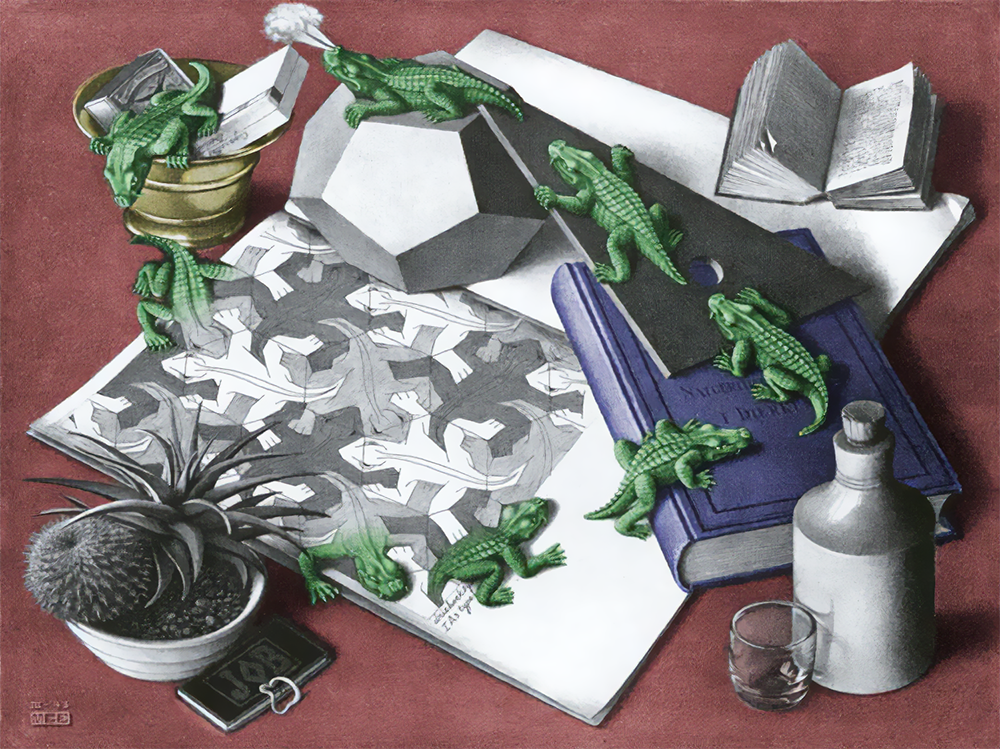
\includegraphics[
        max width=\textwidth,
        max totalheight=\textheight-2\baselineskip
    ]{img/escher-reptiles_colorized.png}
    \caption{М.К.~Эшер «Рептилии»}
    \label{fig:escher-reptiles}
\end{figure}

\speak{Ахилл} И взгляните не наш ли это флакончик с Выталкивающей настойкой там на столе, рядом с ящеричным хороводом?

\speak{Черепаха} Безусловно, это он, Ахилл. Должна сказать, что нам действительно везет. Система обошлась с нами по-божески, вернув нам эту драгоценную жидкость!

\speak{Ахилл} Это верно. Теперь мы можем вытолкнуться из эшеровского мира и вернуться ко мне домой.

\speak{Черепаха} Интересно, что это за книги там, рядом с настойкой? \emph{(Она берет книгу поменьше, открытую в середине.)} Эта книжица выглядит довольно занимательно.

\speak{Ахилл} Правда? Как она называется?

\speak{Черепаха} «Занимательные приключения Черепахи и Ахилла или Вокруг света от точки до точки.» Интересно было было бы почитать немного.

\speak{Ахилл} Вы можете читать, если хотите, а я не собираюсь рисковать, какая-нибудь ящерица может запросто толкнуть флакон и разлить настойку. Я выпью свою порцию немедленно! \emph{(Он бросается к столу и протягивает руку к пузырьку с настойкой; при этом он случайно толкает его. Пузырек падает со стола и катится.)} Ой! Г-жа Ч, смотрите! Я нечаянно столкнул настойку на пол и она покатилась\ldots{} к лестнице! Быстрее, а то свалится вниз!

\direct{\emph{(Но Черепаха погружена в свою книгу.)}}

\speak{Черепаха (бормочет)} А? Эта история выглядит захватывающе.

\speak{Ахилл} Г-жа Ч, скорей, на помощь! Помогите поймать пузырек!

\speak{Черепаха} Что за шум?

\speak{Ахилл} Пузырек с настойкой, я столкнул его со стола, и сейчас он катится, и\ldots{} \emph{(В этот момент пузырек достигает первой ступеньки и падает вниз )} Ох! Что теперь делать? Г-жа Черепаха, вас это не волнует? Мы теряем настойку! Она только что свалилась с лестницы. Единственная наша надежда \--- перейти на другой этаж!

\speak{Черепаха} Перейти на другой рассказ? С превеликим удовольствием! Желаете ко мне присоединиться?

\direct{\emph{(Она начинает читать вслух, Ахилл застывает в нерешительности, не зная, что предпринять. Наконец он решает остаться и начинает читать за Черепаху.)}}

% #endregion

%% BEGIN SUB-LEVEL 3
\begin{sublevel}

% #region Level 3 (first part)

\speak{Ахилл} Как здесь темно, г-жа Ч\@. Я ничего не вижу. Ой! Я натолкнулся на стену. Осторожнее!

\speak{Черепаха} У меня есть пара тросточек. Вот, держите одну. Вы можете прощупывать дорогу, чтобы ни с чем не сталкиваться.

\speak{Ахилл} Отличная идея. \emph{(Он берет трость.)} Вам не кажется, что дорога слегка изгибается влево?

\speak{Черепаха} Да, пожалуй.

\speak{Ахилл} Интересно, где мы находимся. И увидим ли мы когда-нибудь дневной свет опять. Как жаль, что я вас послушался и проглотил эту штуковину «Выпей меня».

\speak{Черепаха} Уверяю вас, она совершенно безвредна. Я делала это много раз и никогда ещё об этом не пожалела. Лучше расслабьтесь и постарайтесь получить удовольствие от того, что вы так чудесно уменьшились.

\speak{Ахилл} Уменьшился? Что вы со мной сделали, г-жа Черепаха?

\speak{Черепаха} Пожалуйста, не обвиняйте меня. Вы проделали все по вашему собственному желанию.

\speak{Ахилл} Так вы меня уменьшили? А вдруг лабиринт, в котором мы находимся, такой крохотный, что кто-нибудь может на него наступить?

\speak{Черепаха} Лабиринт? Лабиринт? Может ли это быть? Неужели мы попали в знаменитый лабиринт ужасного Мажотавра?

\speak{Ахилл} Ой, мамочка! Что это такое?

\speak{Черепаха} Говорят \--- хотя я лично в это никогда не верила \--- что злобный Мажотавр создал миниатюрный лабиринт и сидит в углублении в центре, поджидая невинных жертв, затерявшихся в чудовищно запутанных переходах. Когда они, окончательно заблудившись, забредают в центр, он начинает над ними смеяться, да так громко, что засмеивает их до смерти!

\speak{Ахилл} О боже, не может быть!

\speak{Черепаха} Это только миф. Смелее, Ахилл!

\direct{\emph{(И храбрая парочка осторожно двигается вперед.)}}

\speak{Ахилл} Потрогайте эти стены. Они напоминают сморщенные жестяные листы \--- только все морщины разного размера.

\direct{\emph{(Чтобы подчеркнуть свои слова, он прикладывает конец трости к стене и идет вперед. Трость подпрыгивает на неровностях стены \--- длинный изогнутый коридор, в котором они находятся, наполняется странными звуками.)}}

\speak{Черепаха (встревоженно)} Что это такое?

\speak{Ахилл} Это я веду тросточкой по стене.

\speak{Черепаха} Ох \--- я было подумала, что это рев кровожадного Мажотавра.

\speak{Ахилл} Я думал, вы сказали, что это все выдумки.

\speak{Черепаха} Конечно. Бояться совершенно нечего.

\direct{\emph{(Ахилл снова прикладывает трость к стене и идет вперед. При этом слышна музыка; звуки исходят из того места, где трость прикасается к стене.)}}

\speak{Черепаха} Ох, Ахилл, у меня дурное предчувствие \--- мне кажется, что этот Лабиринт не такой уж и миф.

\speak{Ахилл} Погодите-ка, что это заставило вас так внезапно передумать?

\speak{Черепаха} Слышите эту музыку? \emph{(Чтобы лучше слышать, Ахилл опускает трость, и мелодия прекращается.)} Эй! Поставьте трость обратно! Я хочу послушать конец этой пьесы! \emph{(Ахилл, сбитый с толку, повинуется и музыка возобновляется.)} Благодарю. Теперь я догадалась, где мы находимся.

% \emph{Рис. 25. Критский лабиринт (Итальянская гравюра; школа Финигерры) Из книги У.Г. Маттьюса «Лабиринты: их история и развитие» (W.H. Mattews, Mazes and Labyrinths. Their History and Development.)}
\begin{figure}
    \centering
    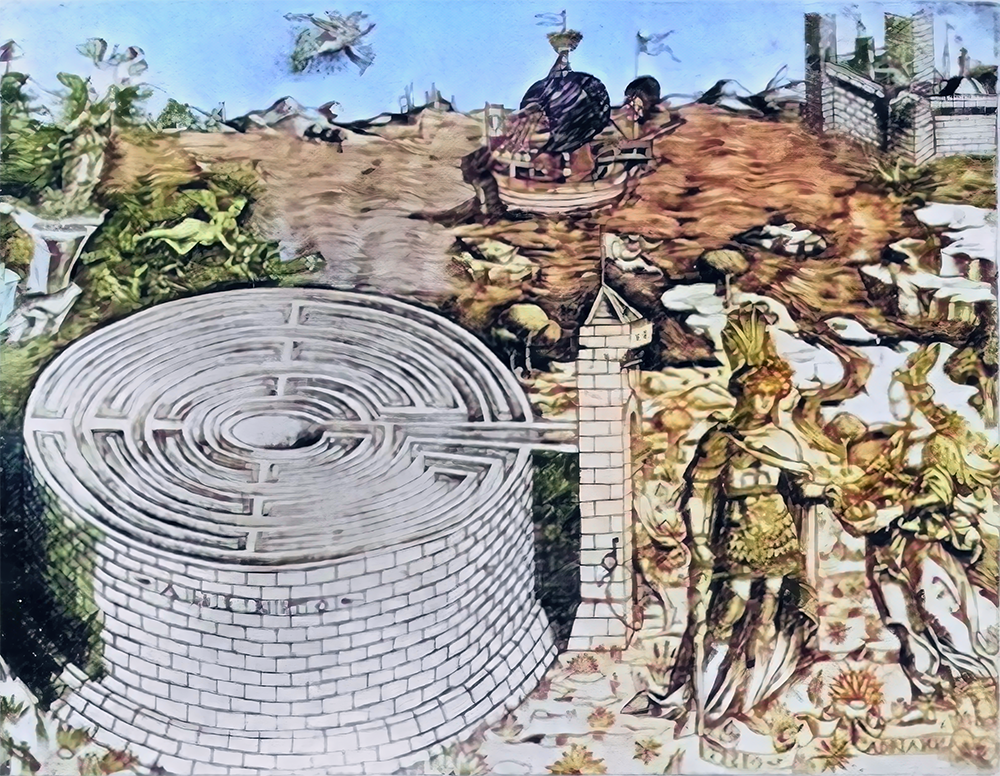
\includegraphics[
        max width=\textwidth,
        max totalheight=\textheight-2\baselineskip
    ]{img/cretan-labyrinth_neuro-color.png}
    \caption{Критский лабиринт}
    \label{fig:cretan-labyrinth}
\end{figure}

\speak{Ахилл} Правда? Где же?

\speak{Черепаха} Мы идем по звуковой дорожке пластинки, лежащей в конверте. Ваша трость, скребущая по морщинам на стене, действует как иголка, бегущая по звуковой дорожке, позволяя нам слушать музыку.

\speak{Ахилл} Ох, нет, нет\ldots{}

\speak{Черепаха} Что такое? Разве вы не радуетесь? Когда ещё вы находились в таком интимном контакте с музыкой?

\speak{Ахилл} Как же я смогу выигрывать соревнования по бегу против людей в натуральную величину, если я теперь меньше блохи, г-жа Черепаха?

\speak{Черепаха} Ах, так вот что вас волнует? Право, Ахилл, стоит ли из-за этого беспокоиться\ldots{}

\speak{Ахилл} Вы говорите так, что у меня создается впечатление, что вы вообще никогда не волнуетесь.

\speak{Черепаха} Не знаю, не знаю\ldots{} Я уверена только в одном: о чем я не жалею, так это о том, что я уменьшилась. В особенности тогда, когда нам грозит страшная опасность от чудовищного Мажотавра.

\speak{Ахилл} О ужас!.. Вы хотите сказать, что\ldots{}

\speak{Черепаха} Боюсь, что да, Ахилл. Музыка выдала его с головой.

\speak{Ахилл} Каким же это образом?

\speak{Черепаха} Очень просто. Когда я услышала мелодию В-А-С-H в верхнем голосе, меня осенило: на звуковых дорожках, по которым мы идем, записано не что иное, как «Маленький гармонический лабиринт», одна из наименее известных органных пьес Баха. Она названа так из-за модуляций, таких частых, что от них начинает кружиться голова.

\speak{Ахилл} Ч-что \--- что это такое и с чем это едят?

\speak{Черепаха} Как вы знаете, большинство музыкальных произведений написано в какой-нибудь тональности \--- например, «до мажор», как эта пьеса.

\speak{Ахилл} Я уже слышал это название раньше. Не правда ли, это значит, что «до» \--- та нота, на которой произведение должно заканчиваться?

\speak{Черепаха} Да, «до» \--- это что-то вроде ключа от дома, куда вы хотите попасть. Ключ бывает и в музыке.

\speak{Ахилл} Значит, сначала мы удаляемся от этого «дома», чтобы потом туда возвратиться?

\speak{Черепаха} Правильно. В музыкальных произведениях часто используются мелодии, уводящие в сторону от ключевой тональности. Мало-помалу нарастает напряжение, и слушатель начинает все сильнее скучать по «дому» \--- ему хочется вновь услышать ключевую тональность.

\speak{Ахилл} Таким образом, в конце пьесы я всегда буду чувствовать такое удовлетворение, как будто я всю жизнь желал услышать именно эти звуки?

\speak{Черепаха} Точно. Композитор использует свои знания о гармонической прогрессии, чтобы таким образом управлять нашими чувствами и пробудить в нас желание услышать ключевую тональность\ldots{}

\speak{Ахилл} Понятно, но, кажется, вы собирались рассказать мне о модуляциях\ldots{}

\speak{Черепаха} Ах, да. Один из важных приемов, которые композитор может использовать где-то в середине пьесы, называется модуляцией; это означает, что он устанавливает временную «цель», отличную от конечного разрешения в ключевую тональность.

\speak{Ахилл} А-а-а\ldots{} кажется, я понимаю. Вы имеете в виду, что определенная серия аккордов изменяет гармоническое напряжение таким образом, что я начинаю желать разрешения в новой тональности?

\speak{Черепаха} Именно так. Это усложняет ситуацию, поскольку, наряду с этим новым желанием, подсознательно вы все время ощущаете, что ваша конечная цель \--- ключевая тональность, в данном случае, «до мажор». И когда временная цель бывает достигнута, то\ldots{}

\speak{Ахилл (внезапно начиная возбужденно жестикулировать)} О, послушайте только: какие восхитительные поднимающиеся вверх аккорды! Какой прекрасный конец у «Маленького гармонического лабиринта»!

\speak{Черепаха} Нет, Ахилл, это не конец, это просто \---

\speak{Ахилл} Да нет, разумеется, это конец! Вот это да! Какой могучий финал! Какое облегчение! Вот разрешение так разрешение! Гениально! \emph{(Поет):} Ля-ля-ля\ldots{} \emph{(И точно, в этот момент музыка прекращается; стен больше нет, и Черепаха с Ахиллом оказываются в открытом пространстве.)} Вот видите, музыка действительно кончилась. Ну, что я вам говорил?

\speak{Черепаха} Что-то здесь не так. Эта запись позорит музыкальный мир.

\speak{Ахилл} Почему это?

\speak{Черепаха} Я только что вам объяснил: Бах промодулировал здесь от «до» в «ля», так что временной целью было услышать мелодию в ключе «ля». Это значит, что вы чувствуете сразу два желания: с одной стороны, вы ожидаете разрешения в «ля», а с другой стороны, вы все время помните, что конечная цель \--- триумфальное возвращение в «до мажор».

\speak{Ахилл} Почему надо все время о чем-то помнить, когда слушаешь музыку? Разве музыка \--- только упражнение для ума?

\speak{Черепаха} Нет, конечно. Некоторые произведения весьма интеллектуальны, но большинство довольно просты. Обычно наше ухо или мозг делают все «расчеты» за нас, в то время как чувства решают, что именно нам хочется услышать. Нам не приходится думать об этом. Но в этой пьесе Бах проделывает разные трюки, в надежде сбить слушателя с толку \--- и надо сказать, что в вашем случае, Ахилл, он вполне преуспел!

\speak{Ахилл} Вы хотите сказать, что я среагировал на разрешение во «второстепенной» тональности?

\speak{Черепаха} Правильно.

\speak{Ахилл} Все же я и сейчас уверен, что это был конец!

\speak{Черепаха} Именно этого эффекта Бах и добивался. Вы угодили прямиком в его ловушку. Это место написано так, что оно звучит как финал; но если вы внимательно следите за развитием гармонической прогрессии, вы увидите, что оно не в том ключе. Видимо, не только вы, но и та несчастная студия звукозаписи решила, что это конец, и записала только часть пьесы!

\speak{Ахилл} Какую недостойную шутку сыграл со мной старик Бах!

\speak{Черепаха} Как раз этого он и хотел \--- заставить вас заблудиться в его «Лабиринте». Видите ли, злодей Мажотавр \--- сообщник Баха. Если вы не остережетесь, он засмеет вас до смерти \--- а может быть, и меня вместе с вами!

\speak{Ахилл} Надо срочно уносить ноги отсюда! Скорее! Если мы побежим обратно по звуковым дорожкам, то выберемся из пластинки прежде, чем страшный Мажотавр нас обнаружит!

\speak{Черепаха} Ну нет, мое ухо слишком чувствительно, чтобы вынести странные аккорды, получающиеся, когда время обращается вспять!

\speak{Ахилл} Ах, г-жа Ч, как же мы выберемся отсюда, если мы не можем вернуться по нашим следам?

\speak{Черепаха} Хороший вопрос\ldots{} \emph{(Почти отчаявшись, Ахилл начинает бегать взад-вперед в темноте. Внезапно раздается сдавленный крик и затем \--- БА-БАХ! \--- глухой звук падения.)} Ахилл? С вами все в порядке?

\speak{Ахилл} Ничего особенного, только маленькая встряска: я свалился в какую-то ямину.

\speak{Черепаха} Вы угодили прямиком в логово Страшного Мажотавра! Постараюсь вас вытащить \--- нам надо удирать побыстрее!

\speak{Ахилл} Осторожнее, г-жа Ч \--- я совсем не хочу, чтобы и Вы тоже попали в западню\ldots{}

\speak{Черепаха} Да не суетитесь вы, Ахилл. Все будет в порядке\ldots{} \emph{(Внезапно раздается сдавленный крик и затем \--- БА-БАХ! \--- глухой звук падения.)}

\speak{Ахилл} Г-жа Ч, вы тоже упали? Не ушиблись?

\speak{Черепаха} Кроме моей гордости, ничего не пострадало.

\speak{Ахилл} Вот теперь мы действительно попали в переплет!

\direct{\emph{(Внезапно, в опасной близости от них, друзья слышат оглушительный хохот.)}}

\speak{Черепаха} Осторожно, Ахилл \--- тут дело нешуточное!

\speak{Мажотавр} Ха-ха-ха! Хи-хи-хи! Хо-хо-хо!

\speak{Ахилл} Я слабею на глазах, г-жа Ч\ldots{}

\speak{Черепаха} Старайтесь не обращать внимания на его смех \--- это ваша единственная надежда.

\speak{Ахилл} Я сделаю все, что в моих силах \--- ах, если бы сейчас пропустить для храбрости рюмочку-другую\ldots{}

\speak{Черепаха} Мне кажется, я чувствую знакомый запах\ldots{} Не вытаскин ли это?

\speak{Ахилл} И правда\ldots{} откуда этот запах?

\speak{Черепаха} По-моему, это здесь\ldots{} О! Я нашла целую бутыль! Это он и есть!

\speak{Ахилл} Вытаскин! Давайте напьемся с горя!

% #endregion

%% Intertext from level 0
\begin{customlevel}{0}
    \speak{Черепаха} Надеюсь, что это не протолкин \--- они до того похожи, что их трудно различить.
\end{customlevel}
%% Return to level 3

\speak{Ахилл} Что вы сказали про Толкиена?

\speak{Черепаха} Я ничего подобного не говорила. У вас уже галлюцинации начинаются\ldots{}

\speak{Ахилл} Б-батюшки мои! Надеюсь, что нет\ldots{} Ну что же, поехали!

\direct{\emph{(И друзья начинают отхлебывать вытаскин (или протолкин?) \--- и вдруг \--- ХЛОП! Кажется, это-таки оказался вытаскин\ldots)}}

%% END SUB-LEVEL 3
\end{sublevel}

% #region Level 2 (third part after sub-3)
\speak{Черепаха} Забавная история, ничего не скажешь. Вам понравилось?

\speak{Ахилл} Так, ничего себе\ldots{} Интересно, выбрались ли они в конце концов из ямы страшного Мажотавра? Бедняга Ахилл, он так хотел опять стать большим.

\speak{Черепаха} Не беспокойтесь \--- они выбрались, и Ахилл снова вырос до своих обычных размеров. Вытаскин оказался весьма кстати\ldots{}

\speak{Ахилл} Не знаю, не знаю\ldots{} Единственное, в чем я сейчас АБСОЛЮТНО уверен, это в том, что нам не мешало бы найти нашу бутылочку с настойкой \--- у меня уже давно горло пересохло. И ничто так не утоляет жажду, как выталкивающая настойка

\speak{Черепаха} Она к тому же известна своим тонизирующим действием. Известны случаи, когда народ просто с ума по ней сходил. Например, когда в начале века продуктовая фабрика Шёнберга перестала производить джин с тоником и начала производство какао, вы не представляете себе, какой из-этого поднялся шум \--- настоящая какаофония!

\speak{Ахилл} Воображаю\ldots{} Но давайте же искать настойку! Погодите \--- взгляните-ка на этих ящериц на столе! Не кажется ли вам, что в них есть что-то необычное?

\speak{Черепаха} Не вижу ничего особенного. А что такое?

\speak{Ахилл} Посмотрите: они вылезают из плоскости картины без помощи выталкивающей настойки! Как они это делают?

\speak{Черепаха} Разве я вам не говорила? Вы можете вылезти из картины, двигаясь перпендикулярно её плоскости. Ящерки научились лезть НАВЕРХ, когда они хотят выбраться из двухмерного мира альбома.

\speak{Ахилл} Может быть, мы можем так же выбраться из этой картины Эшера наружу?

\speak{Черепаха} Разумеется \--- нужно только подняться уровнем выше. Хотите попытаться?

\speak{Ахилл} Все что угодно, только бы попасть домой! Я уже сыт по горло этими занимательными приключениями.

\speak{Черепаха} В таком случае, следуйте за мной наверх.

\direct{\emph{(И они поднимаются на один уровень.)}}

% #endregion

%% END SUB-LEVEL 2
\end{sublevel}

\speak{Ахилл} Хорошо быть снова у себя дома\ldots{} Но постойте, здесь что-то не~то! Это вовсе не мой дом \--- это ВАШ дом, г-жа Черепаха!

\speak{Черепаха} Вы правы \--- и я предовольна, так как перспектива тащиться от вас к себе домой мне совершенно не улыбалась. Я прямо-таки валюсь с лап от усталости.

\speak{Ахилл} Что ж, я как раз не возражаю против небольшой прогулки; так что, мне кажется, все сложилось довольно удачно.

\speak{Черепаха} Я думаю! Вот это удача так удача!

% Note: Dialogue ends on level 1.

%% END SUB-LEVEL 1
\end{sublevel}

\end{Dialogue}

\end{document}
